\section{Méthodologie}
\label{sec:methodologie}

\subsection{Dataset SEED-VIG}

\subsubsection{Description Générale}

Le dataset SEED-VIG (SJTU Emotion EEG Dataset - Vigilance) \cite{zheng2017seedvig} a été conçu spécifiquement pour l'estimation de la vigilance en situation de conduite. Il contient des enregistrements de 23 sujets (18 hommes, 5 femmes, âge moyen : 23.4 $\pm$ 2.1 ans) effectuant une tâche de conduite simulée d'une durée d'environ 2 heures.

\textbf{Caractéristiques principales :}
\begin{itemize}
    \item \textbf{Nombre de sujets :} 23
    \item \textbf{Sessions :} 2 par sujet (midi et nuit)
    \item \textbf{Durée par session :} $\sim$2 heures
    \item \textbf{Échantillonnage temporel :} 885 échantillons par session (fenêtres de 8 secondes)
\end{itemize}

\subsubsection{Protocole Expérimental}

\textbf{Tâche de conduite :}
\begin{enumerate}
    \item Simulation de conduite sur autoroute monotone
    \item Vitesse constante imposée (60 km/h)
    \item Consigne : maintenir le véhicule au centre de la voie
    \item Durée : jusqu'à endormissement ou maximum 2h
\end{enumerate}

\textbf{Conditions expérimentales :}
\begin{itemize}
    \item \textbf{Session "noon" (midi) :} 14h00 - 16h00, après repas (favorise somnolence post-prandiale)
    \item \textbf{Session "night" (nuit) :} 22h00 - 00h00, privation de sommeil partielle
\end{itemize}

\textbf{Enregistrements :}
\begin{itemize}
    \item \textbf{EEG :} 17 électrodes selon système 10-20 international
    \item \textbf{EOG :} 3 électrodes (horizontale, verticale)
    \item \textbf{Caméra :} Enregistrement facial pour calcul du PERCLOS
    \item \textbf{Fréquence d'échantillonnage :} 1000 Hz (réduit à 2 Hz après traitement)
\end{itemize}

\begin{figure}[H]
\centering
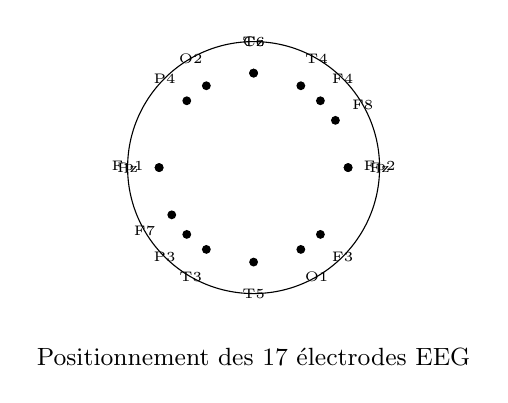
\begin{tikzpicture}[scale=0.8]
% Tête (vue de dessus)
\draw (0,0) circle (2cm);

% Électrodes EEG (système 10-20 simplifié)
\foreach \angle/\label in {0/Fp2, 30/F8, 60/T4, 90/T6, 120/O2, 
                           180/Fp1, 210/F7, 240/T3, 270/T5, 300/O1,
                           45/F4, 135/P4, 225/P3, 315/F3, 
                           0/Fz, 90/Cz, 180/Pz} {
    \fill (\angle:1.5cm) circle (2pt);
    \node at (\angle:2cm) {\tiny \label};
}

\node at (0,-3) {\small Positionnement des 17 électrodes EEG};
\end{tikzpicture}
\caption{Schéma simplifié du positionnement des électrodes EEG (système 10-20)}
\label{fig:electrodes}
\end{figure}

\subsubsection{Variable Cible : PERCLOS}

Le PERCLOS (PERcentage of eye CLOSure) est une mesure objective de la somnolence définie par :

\begin{equation}
\text{PERCLOS} = \frac{\text{Temps où paupières fermées à 80\%}}{\text{Temps total}} \times 100\%
\end{equation}

\textbf{Propriétés :}
\begin{itemize}
    \item Valeurs continues dans $[0, 1]$
    \item PERCLOS $< 0.15$ : Éveillé
    \item PERCLOS $\in [0.15, 0.30]$ : Somnolence modérée
    \item PERCLOS $> 0.30$ : Somnolence sévère
\end{itemize}

Le PERCLOS est calculé automatiquement à partir de l'enregistrement vidéo du visage du conducteur via un algorithme de détection de points faciaux \cite{daza2020driver}.

\subsection{Extraction de Features}

\subsubsection{Prétraitement des Signaux}

\textbf{Pour l'EEG :}
\begin{enumerate}
    \item \textbf{Filtrage :} Passe-bande 0.1-75 Hz, filtre coupe-bande 50 Hz (réduction bruit électrique)
    \item \textbf{Suppression des artéfacts :} Analyse en Composantes Indépendantes (ICA) pour retirer clignements, mouvements musculaires
    \item \textbf{Segmentation :} Fenêtres de 8 secondes sans recouvrement
    \item \textbf{Re-référencement :} Référence moyenne commune (CAR)
\end{enumerate}

\textbf{Pour l'EOG :}
\begin{enumerate}
    \item \textbf{Filtrage :} Passe-bande 0.1-30 Hz
    \item \textbf{Segmentation :} Fenêtres de 8 secondes (synchronisées avec EEG)
\end{enumerate}

\subsubsection{Features EEG : Differential Entropy}

Pour chaque fenêtre de 8 secondes et chaque canal EEG, le DE est calculé pour 5 bandes de fréquence :

\begin{table}[H]
\centering
\caption{Calcul des features DE par bande de fréquence}
\label{tab:de_calculation}
\begin{tabular}{lccc}
\toprule
\textbf{Bande} & \textbf{Fréquence (Hz)} & \textbf{Calcul} & \textbf{Features} \\
\midrule
Delta & 1-4 & $h_\delta = \frac{1}{2}\log(2\pi e\sigma^2_\delta)$ & 17 \\
Theta & 4-8 & $h_\theta = \frac{1}{2}\log(2\pi e\sigma^2_\theta)$ & 17 \\
Alpha & 8-14 & $h_\alpha = \frac{1}{2}\log(2\pi e\sigma^2_\alpha)$ & 17 \\
Beta & 14-31 & $h_\beta = \frac{1}{2}\log(2\pi e\sigma^2_\beta)$ & 17 \\
Gamma & 31-50 & $h_\gamma = \frac{1}{2}\log(2\pi e\sigma^2_\gamma)$ & 17 \\
\midrule
\multicolumn{3}{r}{\textbf{Total EEG (avant LDS) :}} & \textbf{85} \\
\bottomrule
\end{tabular}
\end{table}

\textbf{Application du lissage LDS :}

Le lissage LDS est appliqué sur les features DE pour réduire le bruit temporel :
\begin{enumerate}
    \item Estimation des paramètres du modèle LDS par maximum de vraisemblance
    \item Application du filtre de Kalman avant-arrière (forward-backward)
    \item Concaténation des features originales et lissées
\end{enumerate}

\textbf{Résultat :} $85 \times 3 + 10 = 275$ features EEG par fenêtre temporelle

\subsubsection{Features EOG}

36 features sont extraites des signaux EOG pour caractériser les mouvements oculaires \cite{hu2013driving} :

\begin{table}[H]
\centering
\caption{Features EOG extraites}
\label{tab:eog_features}
\begin{tabular}{llc}
\toprule
\textbf{Type} & \textbf{Statistique} & \textbf{Nombre} \\
\midrule
\multirow{3}{*}{Clignements} & Taux (max, moyen, somme) & 3 \\
 & Amplitude (max, moyenne, somme) & 3 \\
 & Durée (max, min, moyenne) & 3 \\
\midrule
\multirow{3}{*}{Saccades} & Taux (max, moyen, somme) & 3 \\
 & Amplitude (max, moyenne, somme) & 3 \\
 & Durée (max, min, moyenne) & 3 \\
\midrule
\multicolumn{2}{l}{\textbf{Total EOG :}} & \textbf{36} \\
\bottomrule
\end{tabular}
\end{table}

\textbf{Détection automatique :}
\begin{itemize}
    \item \textbf{Clignements :} Pics négatifs dépassant un seuil adaptatif (amplitude $> 100\mu V$, durée 100-400 ms)
    \item \textbf{Saccades :} Variations rapides du signal EOG horizontal (vitesse $> 30°$/s)
\end{itemize}

\subsubsection{Vecteur de Features Final}

Pour chaque fenêtre temporelle de 8 secondes :

\begin{equation}
\mathbf{x}_t = [\mathbf{x}_t^{\text{EEG}}; \mathbf{x}_t^{\text{EOG}}] \in \mathbb{R}^{311}
\end{equation}

où :
\begin{itemize}
    \item $\mathbf{x}_t^{\text{EEG}} \in \mathbb{R}^{275}$ : Features DE avec lissage LDS
    \item $\mathbf{x}_t^{\text{EOG}} \in \mathbb{R}^{36}$ : Features mouvements oculaires
\end{itemize}

\textbf{Note importante :} Dans notre implémentation, nous utilisons uniquement les canaux EEG \textbf{postérieurs} (électrodes 7 à 17 du système 10-20), réduisant les features EEG de 275 à 275 (ce point sera précisé dans la section implémentation).

\subsection{Modèles d'Estimation}

\subsubsection{Support Vector Regression (SVR)}

\textbf{Formulation du problème :}

Étant donné un ensemble d'entraînement $\{(\mathbf{x}_i, y_i)\}_{i=1}^n$, le SVR cherche une fonction $f(\mathbf{x}) = \mathbf{w}^T\phi(\mathbf{x}) + b$ qui approxime $y$ avec une erreur maximale $\epsilon$.

\textbf{Problème d'optimisation (forme primale) :}
\begin{equation}
\begin{aligned}
\min_{\mathbf{w},b,\xi,\xi^*} \quad & \frac{1}{2}\|\mathbf{w}\|^2 + C\sum_{i=1}^n(\xi_i + \xi_i^*) \\
\text{s.t.} \quad & y_i - (\mathbf{w}^T\phi(\mathbf{x}_i) + b) \leq \epsilon + \xi_i \\
& (\mathbf{w}^T\phi(\mathbf{x}_i) + b) - y_i \leq \epsilon + \xi_i^* \\
& \xi_i, \xi_i^* \geq 0
\end{aligned}
\end{equation}

\textbf{Solution duale :}
\begin{equation}
f(\mathbf{x}) = \sum_{i=1}^n (\alpha_i - \alpha_i^*)K(\mathbf{x}_i, \mathbf{x}) + b
\end{equation}

où $K(\mathbf{x}_i, \mathbf{x}_j)$ est une fonction noyau.

\textbf{Noyau RBF (Radial Basis Function) :}
\begin{equation}
K(\mathbf{x}_i, \mathbf{x}_j) = \exp\left(-\gamma\|\mathbf{x}_i - \mathbf{x}_j\|^2\right)
\end{equation}

\textbf{Hyperparamètres :}
\begin{itemize}
    \item $C$ : Paramètre de régularisation (compromis complexité/erreur)
    \item $\gamma$ : Paramètre du noyau RBF (largeur de la gaussienne)
    \item $\epsilon$ : Marge d'erreur tolérée
\end{itemize}

\textbf{Interprétation pour la vigilance :}

Le SVR traite chaque instant $t$ de manière indépendante :
\begin{equation}
\hat{y}_t = f(\mathbf{x}_t)
\end{equation}

Il n'y a \textbf{pas de modélisation explicite} de la cohérence temporelle entre $\hat{y}_t$ et $\hat{y}_{t-1}$.

\subsubsection{Continuous Conditional Random Field (CCRF)}

\textbf{Motivation :}

La vigilance évolue de manière continue et cohérente dans le temps. Un conducteur ne passe pas instantanément de "totalement éveillé" à "totalement endormi". Le CCRF modélise cette cohérence temporelle.

\textbf{Modèle graphique :}

Pour une séquence $\mathbf{X} = (\mathbf{x}_1, \ldots, \mathbf{x}_T)$ et $\mathbf{y} = (y_1, \ldots, y_T)$ :

\begin{figure}[H]
\centering
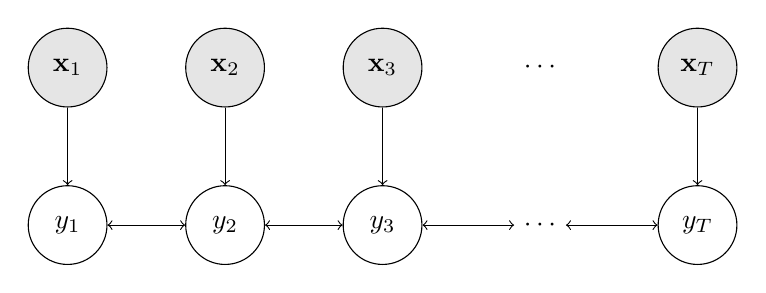
\begin{tikzpicture}[
    node distance=2cm,
    obs/.style={circle, draw, fill=gray!20, minimum size=1cm},
    latent/.style={circle, draw, minimum size=1cm}
]
% Observations
\node[obs] (x1) {$\mathbf{x}_1$};
\node[obs, right of=x1] (x2) {$\mathbf{x}_2$};
\node[obs, right of=x2] (x3) {$\mathbf{x}_3$};
\node[right of=x3] (xdots) {$\cdots$};
\node[obs, right of=xdots] (xT) {$\mathbf{x}_T$};

% Variables de sortie
\node[latent, below of=x1] (y1) {$y_1$};
\node[latent, below of=x2] (y2) {$y_2$};
\node[latent, below of=x3] (y3) {$y_3$};
\node[below of=xdots] (ydots) {$\cdots$};
\node[latent, below of=xT] (yT) {$y_T$};

% Arêtes
\draw[->] (x1) -- (y1);
\draw[->] (x2) -- (y2);
\draw[->] (x3) -- (y3);
\draw[->] (xT) -- (yT);
\draw[<->] (y1) -- (y2);
\draw[<->] (y2) -- (y3);
\draw[<->] (y3) -- (ydots);
\draw[<->] (ydots) -- (yT);

\end{tikzpicture}
\caption{Structure graphique du CCRF : les observations $\mathbf{x}_t$ influencent les sorties $y_t$, et les sorties sont corrélées temporellement}
\label{fig:ccrf_graph}
\end{figure}

\textbf{Distribution de probabilité :}
\begin{equation}
P(\mathbf{y}|\mathbf{X}) = \frac{1}{Z(\mathbf{X})}\exp\left(\sum_{t=1}^T\Phi(y_t,\mathbf{x}_t) + \sum_{t=2}^T\Psi(y_t,y_{t-1})\right)
\label{eq:ccrf}
\end{equation}

\textbf{Potentiel unaire} (relation observation-sortie) :
\begin{equation}
\Phi(y_t,\mathbf{x}_t) = \mathbf{w}^T\mathbf{x}_t \cdot y_t - \frac{1}{2}y_t^2
\end{equation}

\textbf{Potentiel d'arête} (cohérence temporelle) :
\begin{equation}
\Psi(y_t,y_{t-1}) = -\lambda(y_t - y_{t-1})^2
\end{equation}

où $\lambda$ est un hyperparamètre contrôlant la force du lissage temporel.

\textbf{Inférence :}

Pour prédire $\mathbf{y}$ étant donné $\mathbf{X}$, on maximise la probabilité a posteriori :
\begin{equation}
\hat{\mathbf{y}} = \argmax_{\mathbf{y}} P(\mathbf{y}|\mathbf{X})
\end{equation}

Cette optimisation peut être résolue efficacement par l'algorithme de Viterbi adapté aux sorties continues.

\textbf{Apprentissage :}

Les paramètres $\mathbf{w}$ et $\lambda$ sont appris par maximum de vraisemblance :
\begin{equation}
\max_{\mathbf{w},\lambda} \sum_{i=1}^n \log P(\mathbf{y}^{(i)}|\mathbf{X}^{(i)}; \mathbf{w}, \lambda)
\end{equation}

résolu par descente de gradient.

\subsubsection{Continuous Conditional Neural Field (CCNF)}

\textbf{Extension du CCRF :}

Le CCNF remplace le potentiel unaire linéaire par un réseau de neurones pour capturer des relations non-linéaires :

\begin{equation}
\Phi(y_t,\mathbf{x}_t) = \sum_{j=1}^J \alpha_j \sigma(\mathbf{w}_j^T\mathbf{x}_t + b_j) \cdot \exp\left(-\frac{(y_t - \mu_j)^2}{2\sigma_j^2}\right)
\end{equation}

où :
\begin{itemize}
    \item $\sigma$ : Fonction d'activation (ReLU, tanh, sigmoïde)
    \item $J$ : Nombre de neurones dans la couche cachée
    \item $\alpha_j, \mathbf{w}_j, b_j, \mu_j, \sigma_j$ : Paramètres à apprendre
\end{itemize}

\textbf{Architecture :}

\begin{figure}[H]
\centering
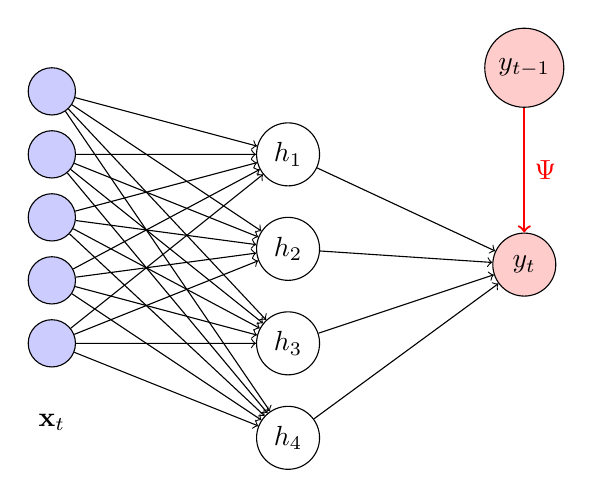
\begin{tikzpicture}[
    neuron/.style={circle, draw, minimum size=0.8cm},
    input/.style={circle, draw, fill=blue!20, minimum size=0.6cm},
    output/.style={circle, draw, fill=red!20, minimum size=0.8cm}
]
% Entrées
\foreach \i in {1,2,3,4,5} {
    \node[input] (x\i) at (0,-\i*0.8) {};
}
\node at (0,-5) {$\mathbf{x}_t$};

% Couche cachée
\foreach \i in {1,2,3,4} {
    \node[neuron] (h\i) at (3,-\i*1.2-0.4) {$h_\i$};
}

% Sortie
\node[output] (y) at (6,-3) {$y_t$};

% Connexions
\foreach \i in {1,2,3,4,5} {
    \foreach \j in {1,2,3,4} {
        \draw[->] (x\i) -- (h\j);
    }
}
\foreach \i in {1,2,3,4} {
    \draw[->] (h\i) -- (y);
}

% Lien temporel
\node[output] (yprev) at (6,-0.5) {$y_{t-1}$};
\draw[->, thick, red] (yprev) -- (y) node[midway, right] {$\Psi$};

\end{tikzpicture}
\caption{Architecture du CCNF : réseau de neurones pour le potentiel unaire + liaison temporelle}
\label{fig:ccnf_arch}
\end{figure}

\textbf{Avantages par rapport au CCRF :}
\begin{enumerate}
    \item Capture des interactions non-linéaires complexes entre features
    \item Représentation distribuée plus riche
    \item Performances empiriques supérieures
\end{enumerate}

\subsection{Protocole d'Évaluation}

\subsubsection{Validation Croisée}

Pour chaque sujet, nous appliquons une validation croisée stratifiée à 5 folds :

\begin{enumerate}
    \item Division de la séquence temporelle en 5 segments contigus
    \item Pour chaque fold $k \in \{1,\ldots,5\}$ :
    \begin{itemize}
        \item Entraînement sur 4 folds (80\% des données)
        \item Test sur 1 fold (20\% des données)
    \end{itemize}
    \item Calcul des métriques sur chaque fold
    \item Moyenne des métriques sur les 5 folds
\end{enumerate}

\textbf{Note :} La division est temporelle (et non aléatoire) pour préserver la structure séquentielle des données.

\subsubsection{Métriques d'Évaluation}

\textbf{1. Coefficient de Corrélation de Pearson (COR) :}

\begin{equation}
\text{COR}(\mathbf{y}, \hat{\mathbf{y}}) = \frac{\sum_{i=1}^n (y_i - \bar{y})(\hat{y}_i - \bar{\hat{y}})}{\sqrt{\sum_{i=1}^n (y_i - \bar{y})^2}\sqrt{\sum_{i=1}^n (\hat{y}_i - \bar{\hat{y}})^2}}
\end{equation}

\textbf{Interprétation :}
\begin{itemize}
    \item COR $\in [-1, 1]$
    \item COR proche de 1 : Excellente corrélation positive
    \item COR $> 0.7$ : Corrélation forte (acceptable)
    \item COR $> 0.8$ : Corrélation très forte (excellent)
\end{itemize}

\textbf{Avantage :} Mesure la capacité à capturer les \textbf{tendances} de la vigilance, indépendamment de l'échelle.

\textbf{2. Root Mean Square Error (RMSE) :}

\begin{equation}
\text{RMSE}(\mathbf{y}, \hat{\mathbf{y}}) = \sqrt{\frac{1}{n}\sum_{i=1}^n (y_i - \hat{y}_i)^2}
\end{equation}

\textbf{Interprétation :}
\begin{itemize}
    \item RMSE $\geq 0$
    \item RMSE petit : Bonnes prédictions absolues
    \item Unité : Même que $y$ (ici, PERCLOS $\in [0,1]$)
\end{itemize}

\textbf{Avantage :} Mesure l'\textbf{erreur absolue} des prédictions.

\textbf{Complémentarité COR/RMSE :}

Un modèle peut avoir un COR élevé (bonnes tendances) mais un RMSE élevé (biais systématique), ou inversement. Les deux métriques sont nécessaires pour une évaluation complète.

\subsubsection{Agrégation des Résultats}

Pour chaque modèle :

\begin{enumerate}
    \item \textbf{Par fold :} Calcul COR et RMSE sur les prédictions du fold
    
    \item \textbf{Moyenne par sujet :}
    \begin{align}
    \text{COR}_{\text{sujet}} &= \frac{1}{5}\sum_{k=1}^5 \text{COR}_k \\
    \text{RMSE}_{\text{sujet}} &= \frac{1}{5}\sum_{k=1}^5 \text{RMSE}_k
    \end{align}
    
    \item \textbf{COR global par sujet :} Concaténation de toutes les prédictions des 5 folds et calcul du COR global (plus robuste)
    
    \item \textbf{Moyenne sur tous les sujets :}
    \begin{align}
    \text{COR}_{\text{global}} &= \frac{1}{23}\sum_{s=1}^{23} \text{COR}_{\text{sujet}}(s) \\
    \text{RMSE}_{\text{global}} &= \frac{1}{23}\sum_{s=1}^{23} \text{RMSE}_{\text{sujet}}(s)
    \end{align}
\end{enumerate}